\section{Scheduling in Model-Based Embedded Design Tools}
\label{integration}

\begin{figure}
		%[height=50mm,width=50mm]
		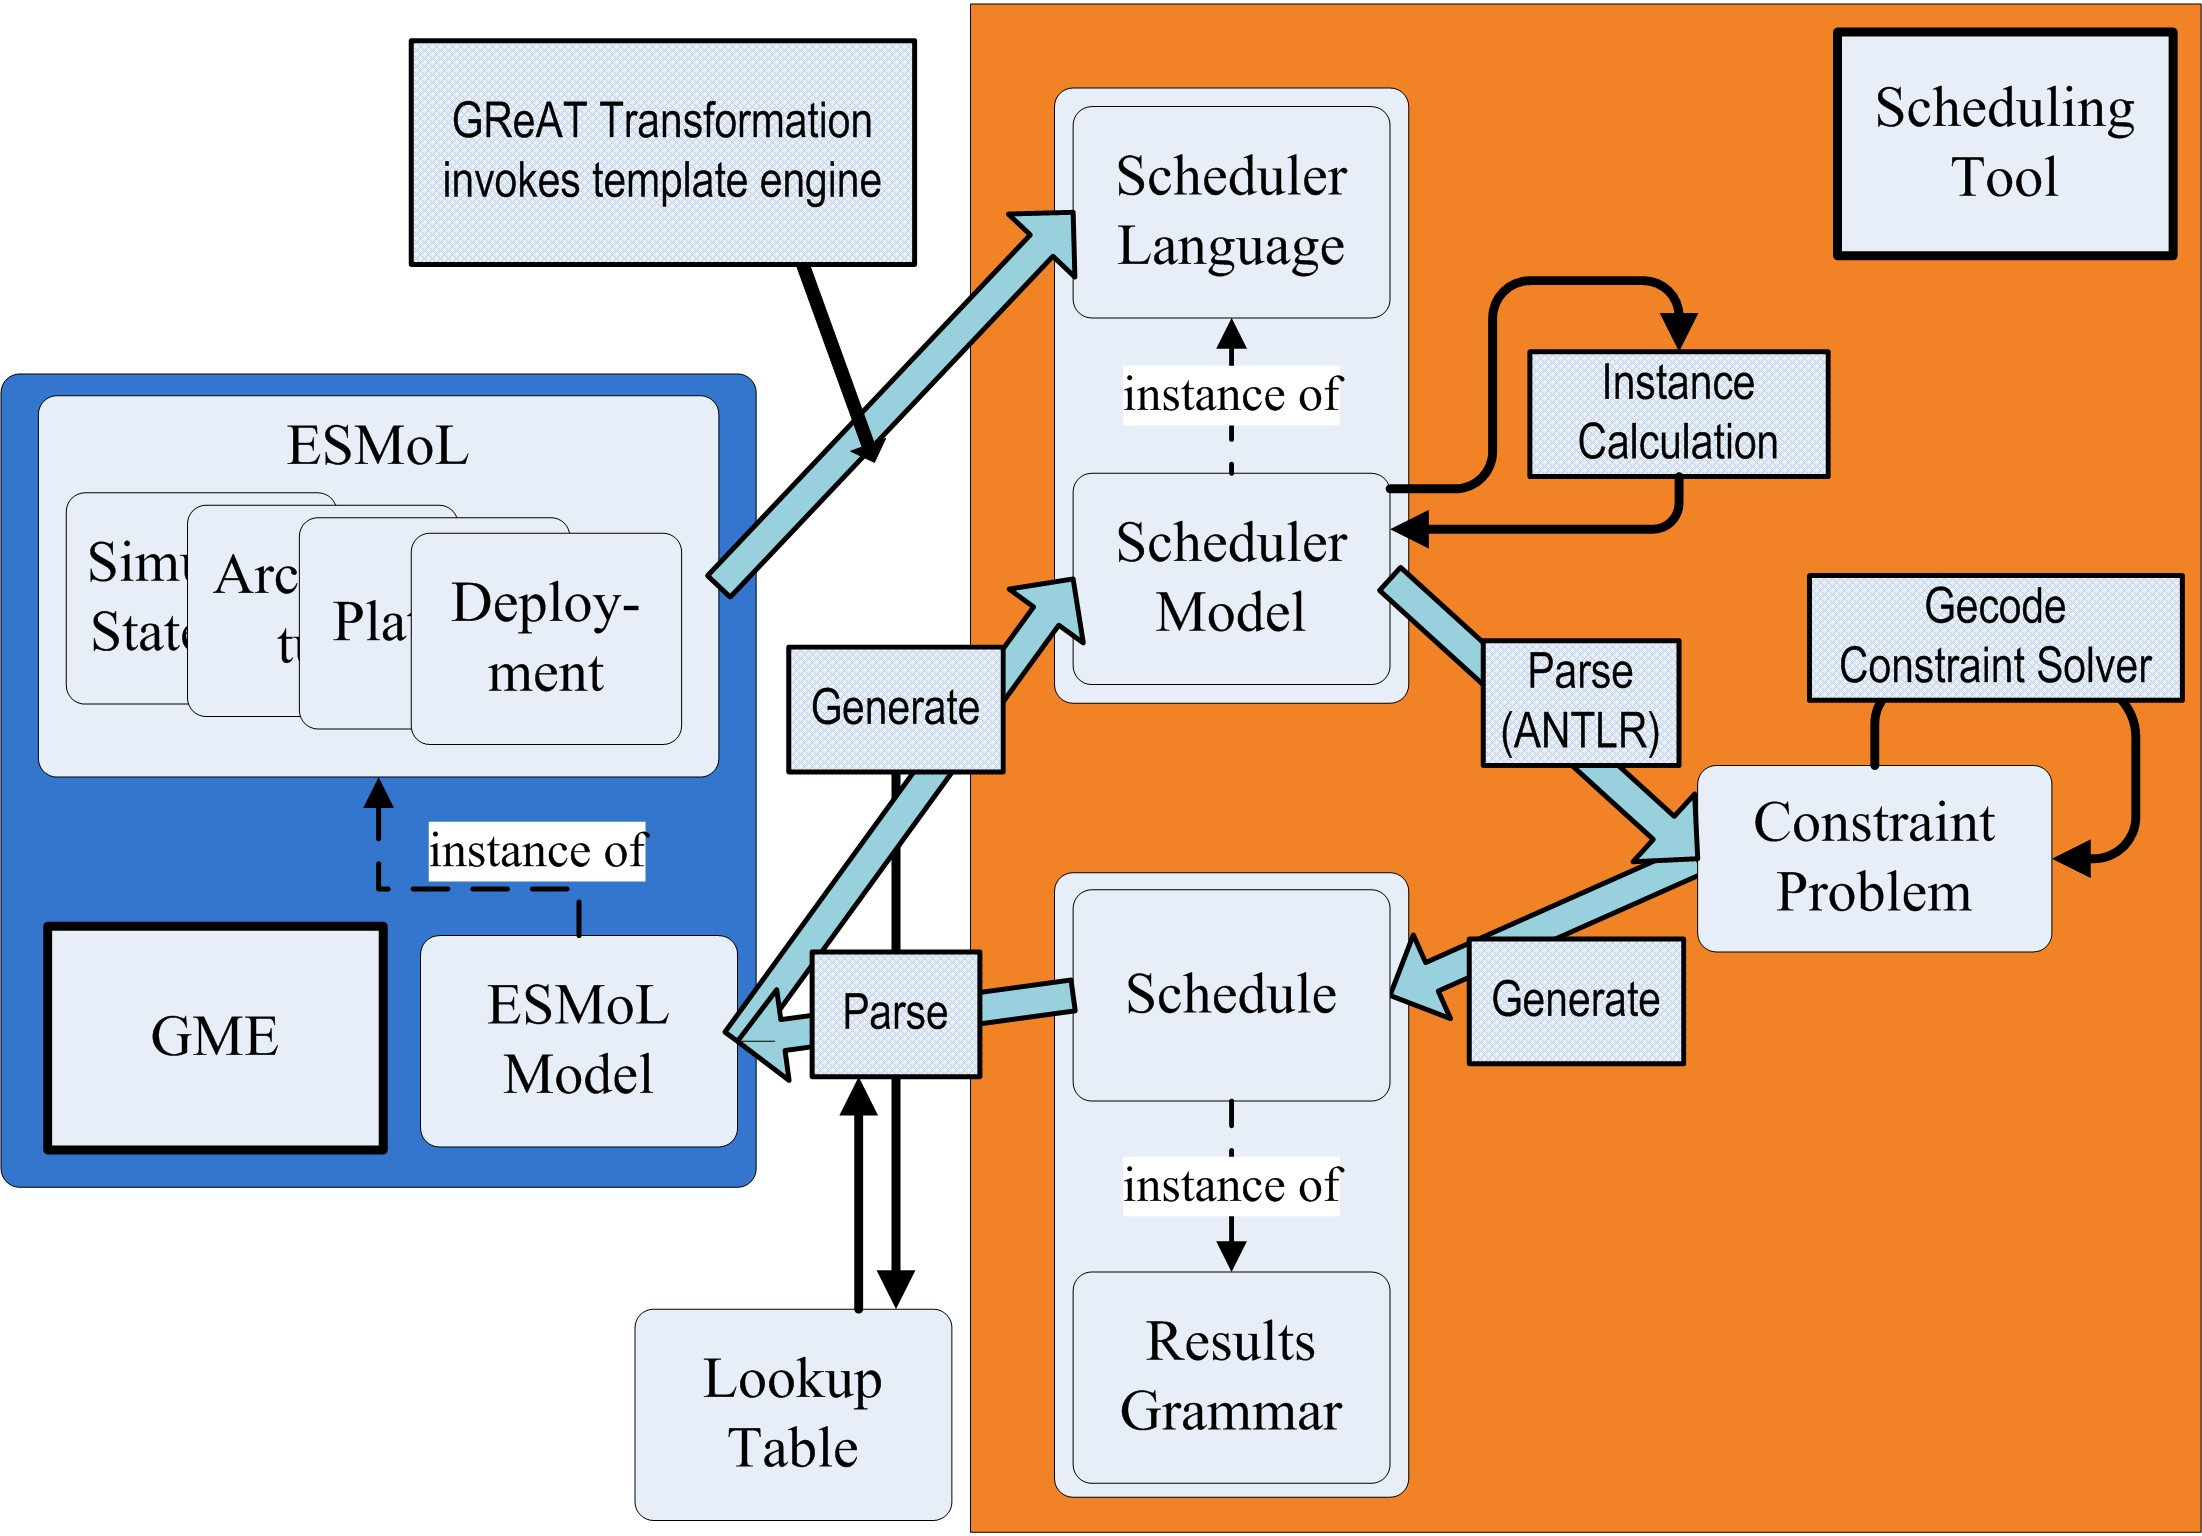
\includegraphics[scale=.9]{figures/adapter.jpg}
		\centering
	  \label{fig:adapter}
		\caption{Integration of Scheduling Tool into Model-Based Embedded Software Design Toolchain}
\end{figure}

ESched was created as part of the ESMoL modeling language and embedded software design suite\cite{modeling:aces08}.  A modeler imports Simulink/Stateflow models\cite{tools:mathworks} into the ESMoL language, adds architecture, platform design, and deployment concepts, and then synthesizes code for execution on a time-triggered network.  The suite includes a portable time-triggered virtual machine\cite{timed:frodo} which can run on generic Linux or FreeRTOS to implement timed execution of tasks and messages.  Execution requires computation of a cyclic schedule for the distributed system.

%\ref{fig:adapter}
Fig. 7 illustrates the language integration of the scheduler with the modeling tool using the model-integrated computing (MIC) tool suite\cite{mic:overview}.  The MIC tools include a graphical modeling/meta-modeling environment (GME\cite{mic:gme}) as well as a model-based graph transformation tool (GReAT\cite{mic:GReAT}).  The ESMoL deployment model elements map directly (syntactically and semantically) to the schedule specification language.  The tools also parse generated schedules and write the start times back into the model for use in platform-specific code configuration.  Extensions currently in development in the tool suite include generation of platform-specific time-triggered simulations in Simulink, using the TrueTime toolkit(\cite{tools:truetime}).  The simulation also requires the computation of a schedule.


